% SonicVitals -- system architecture (vector figure, compiled to PDF and
% included by SonicVitals_Journal_Paper.tex).
% Build:  pdflatex fig_architecture.tex
%
% Blocks drawn with the "planned" style (dashed amber outline) belong to the
% target design but are NOT yet implemented in the repository. Once the code
% matches the paper, change \markplannedtrue to \markplannedfalse and rebuild.
\documentclass[tikz,border=4pt]{standalone}
\usepackage{amsmath}
\usepackage{newtxtext,newtxmath}
\usetikzlibrary{arrows.meta,positioning,calc,fit,backgrounds}

\newif\ifmarkplanned
\markplannedfalse

\definecolor{navy}{RGB}{0,40,85}
\definecolor{blue}{RGB}{0,98,155}
\definecolor{tierfill}{RGB}{238,244,250}
\definecolor{green}{RGB}{0,128,80}
\definecolor{amber}{RGB}{200,110,20}

\ifmarkplanned
  \tikzset{planned/.style={dashed, draw=amber}}
\else
  \tikzset{planned/.style={}}
\fi

\begin{document}
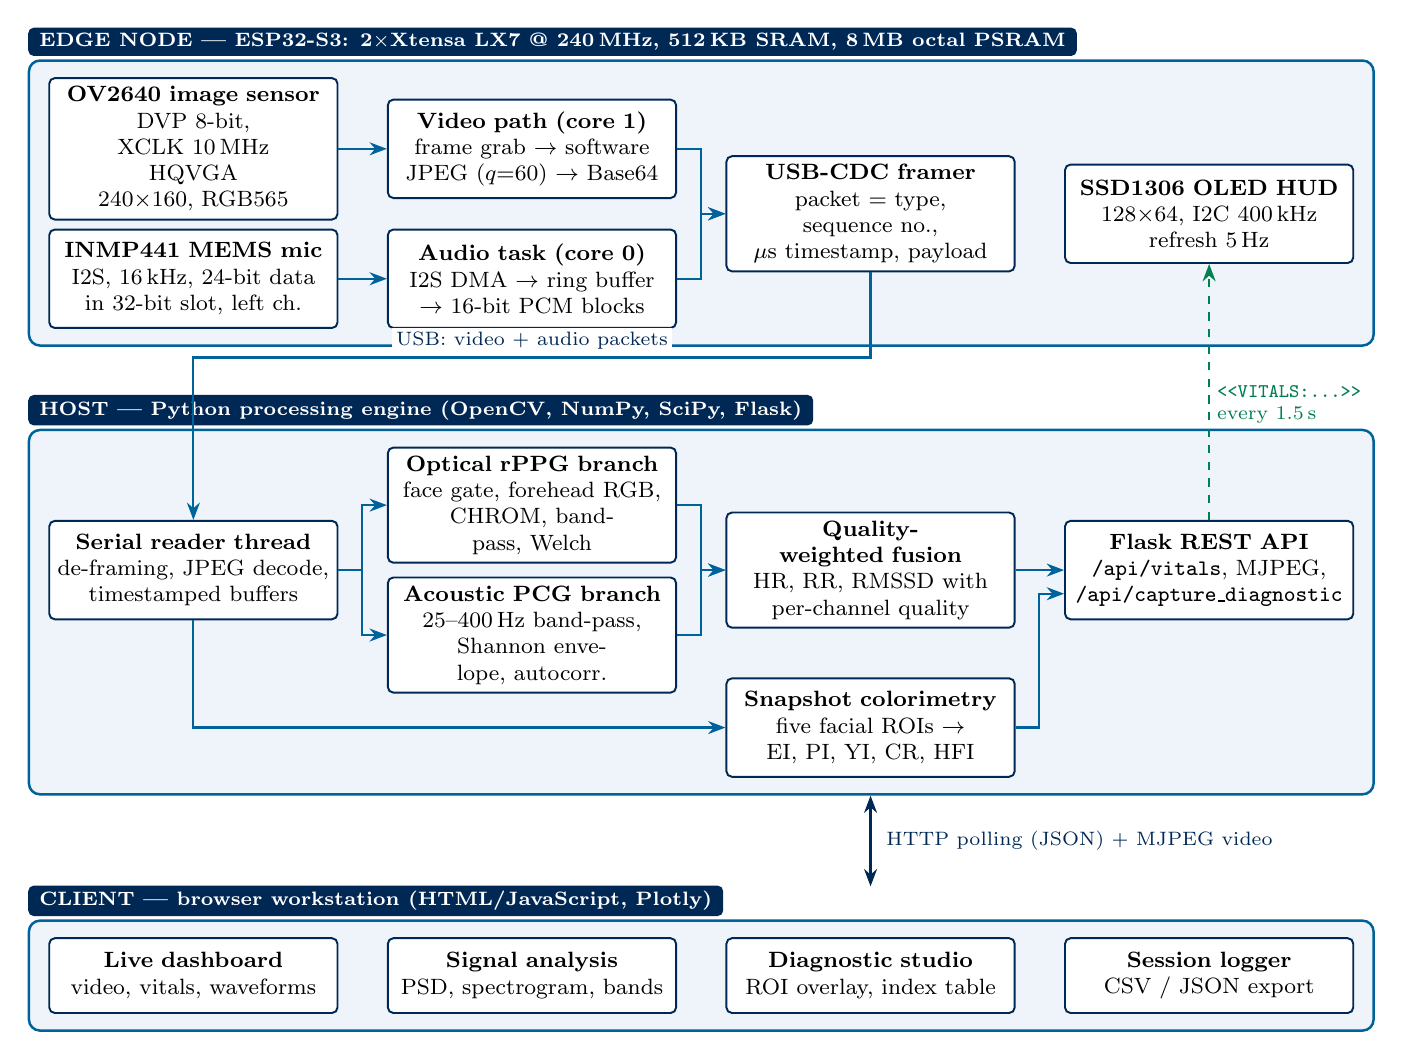
\begin{tikzpicture}[
  font=\footnotesize,
  >={Stealth[length=2.2mm]},
  blk/.style={draw=navy, fill=white, rounded corners=2pt, line width=0.7pt,
              align=center, inner sep=3pt, text width=3.45cm, minimum height=1.25cm},
  tier/.style={draw=blue, fill=tierfill, rounded corners=4pt, line width=0.9pt,
               inner xsep=7pt, inner ysep=6pt},
  tiertitle/.style={fill=navy, text=white, font=\scriptsize\bfseries,
                    rounded corners=2pt, inner xsep=4pt, inner ysep=2pt, anchor=south west},
  data/.style={->, line width=0.8pt, draw=blue},
  ctrl/.style={->, line width=0.8pt, draw=green, dashed},
  lbl/.style={font=\scriptsize, text=navy, fill=tierfill, inner sep=1.5pt}
]
\def\cA{0} \def\cB{4.3} \def\cC{8.6} \def\cD{12.9}

% ================================================================ EDGE NODE
\node[blk] (cam) at (\cA,0)
  {\textbf{OV2640 image sensor}\\ DVP 8-bit, XCLK 10\,MHz\\ HQVGA $240{\times}160$, RGB565};
\node[blk] (mic) at (\cA,-1.65)
  {\textbf{INMP441 MEMS mic}\\ I2S, 16\,kHz, 24-bit data\\ in 32-bit slot, left ch.};
\node[blk] (vid) at (\cB,0)
  {\textbf{Video path (core 1)}\\ frame grab $\rightarrow$ software\\ JPEG ($q{=}60$) $\rightarrow$ Base64};
\node[blk, planned] (aud) at (\cB,-1.65)
  {\textbf{Audio task (core 0)}\\ I2S DMA $\rightarrow$ ring buffer\\ $\rightarrow$ 16-bit PCM blocks};
\node[blk, planned] (frm) at (\cC,-0.825)
  {\textbf{USB-CDC framer}\\ packet = type, sequence no.,\\ $\mu$s timestamp, payload};
\node[blk] (oled) at (\cD,-0.825)
  {\textbf{SSD1306 OLED HUD}\\ $128{\times}64$, I2C 400\,kHz\\ refresh 5\,Hz};

\draw[data] (cam) -- (vid);
\draw[data] (mic) -- (aud);
\draw[data] (vid.east) -- ++(0.3,0) |- (frm.west);
\draw[data] (aud.east) -- ++(0.3,0) |- (frm.west);

\begin{scope}[on background layer]
  \node[tier, fit=(cam)(mic)(oled)] (t1) {};
\end{scope}
\node[tiertitle] at ([yshift=1pt]t1.north west)
  {EDGE NODE --- ESP32-S3: 2$\times$Xtensa LX7 @ 240\,MHz, 512\,KB SRAM, 8\,MB octal PSRAM};

% ================================================================ HOST
\def\yH{-5.35}
\node[blk] (rdr) at (\cA,\yH)
  {\textbf{Serial reader thread}\\ de-framing, JPEG decode,\\ timestamped buffers};
\node[blk] (opt) at (\cB,\yH+0.825)
  {\textbf{Optical rPPG branch}\\ face gate, forehead RGB,\\ CHROM, band-pass, Welch};
\node[blk, planned] (aco) at (\cB,\yH-0.825)
  {\textbf{Acoustic PCG branch}\\ 25--400\,Hz band-pass,\\ Shannon envelope, autocorr.};
\node[blk, planned] (fus) at (\cC,\yH)
  {\textbf{Quality-weighted fusion}\\ HR, RR, RMSSD with\\ per-channel quality};
\node[blk] (api) at (\cD,\yH)
  {\textbf{Flask REST API}\\ \texttt{/api/vitals}, MJPEG,\\ \texttt{/api/capture\_diagnostic}};
\node[blk] (col) at (\cC,\yH-2.0)
  {\textbf{Snapshot colorimetry}\\ five facial ROIs $\rightarrow$\\ EI, PI, YI, CR, HFI};

\draw[data] (rdr.east) -- ++(0.3,0) |- (opt.west);
\draw[data] (rdr.east) -- ++(0.3,0) |- (aco.west);
\draw[data] (opt.east) -- ++(0.3,0) |- (fus.west);
\draw[data] (aco.east) -- ++(0.3,0) |- (fus.west);
\draw[data] (fus) -- (api);
\draw[data] (col.east) -- ++(0.3,0) |- ([yshift=-0.3cm]api.west);
\draw[data] (rdr.south) |- (col.west);

\begin{scope}[on background layer]
  \node[tier, fit=(rdr)(opt)(col)(api)] (t2) {};
\end{scope}
\node[tiertitle] at ([yshift=1pt]t2.north west)
  {HOST --- Python processing engine (OpenCV, NumPy, SciPy, Flask)};

% ================================================================ CLIENT
\def\yC{-10.5}
\node[blk, minimum height=0.95cm] (u1) at (\cA,\yC) {\textbf{Live dashboard}\\ video, vitals, waveforms};
\node[blk, minimum height=0.95cm] (u2) at (\cB,\yC) {\textbf{Signal analysis}\\ PSD, spectrogram, bands};
\node[blk, minimum height=0.95cm] (u3) at (\cC,\yC) {\textbf{Diagnostic studio}\\ ROI overlay, index table};
\node[blk, minimum height=0.95cm] (u4) at (\cD,\yC) {\textbf{Session logger}\\ CSV / JSON export};

\begin{scope}[on background layer]
  \node[tier, fit=(u1)(u4)] (t3) {};
\end{scope}
\node[tiertitle] at ([yshift=1pt]t3.north west)
  {CLIENT --- browser workstation (HTML/JavaScript, Plotly)};

% ================================================================ LINKS
\draw[data] (frm.south) -- (\cC,-2.65) -| (rdr.north)
  node[lbl, pos=0.25, above=1pt, fill=white] {USB: video + audio packets};
\draw[ctrl] (api.north) -- (oled.south)
  node[pos=0.45, right=1pt, font=\scriptsize, text=green, align=left, fill=white, inner sep=1.5pt]
  {\texttt{<<VITALS:...>>}\\every 1.5\,s};
\draw[<->, line width=0.8pt, draw=navy] ([xshift=2.15cm]t2.south) -- ([xshift=2.15cm, yshift=0.42cm]t3.north)
  node[midway, right=2pt, font=\scriptsize, text=navy] {HTTP polling (JSON) + MJPEG video};

\ifmarkplanned
\node[anchor=north east, font=\scriptsize] at ([yshift=-3pt]t3.south east)
  {\tikz[baseline=-0.6ex]{\draw[amber,dashed,line width=0.7pt,rounded corners=1pt] (0,-0.1) rectangle (0.55,0.12);}
   \ planned in target design, not yet implemented};
\fi
\end{tikzpicture}
\end{document}
